\chapter{Planung und Aufwand} \label{Planung und Aufwand}

Nach Fertigstellung des Architektur-Entwurfs wurde zunächst der Aufwand für die verschiedenen Implementierungsschritte geschätzt und eine sinnvolle Reihenfolge für die Implementierung der verschiedenen Komponenten festgelegt.
Die hier dargestellten Gantt-Diagramme geben einen groben Überblick des geplanten und tatsächlichen Ablaufs.
Außerdem wird eine Gegenüberstellung des erwarteten und tatsächlichen Implementierungs-Aufwands in Stunden gegeben.


\begin{figure}
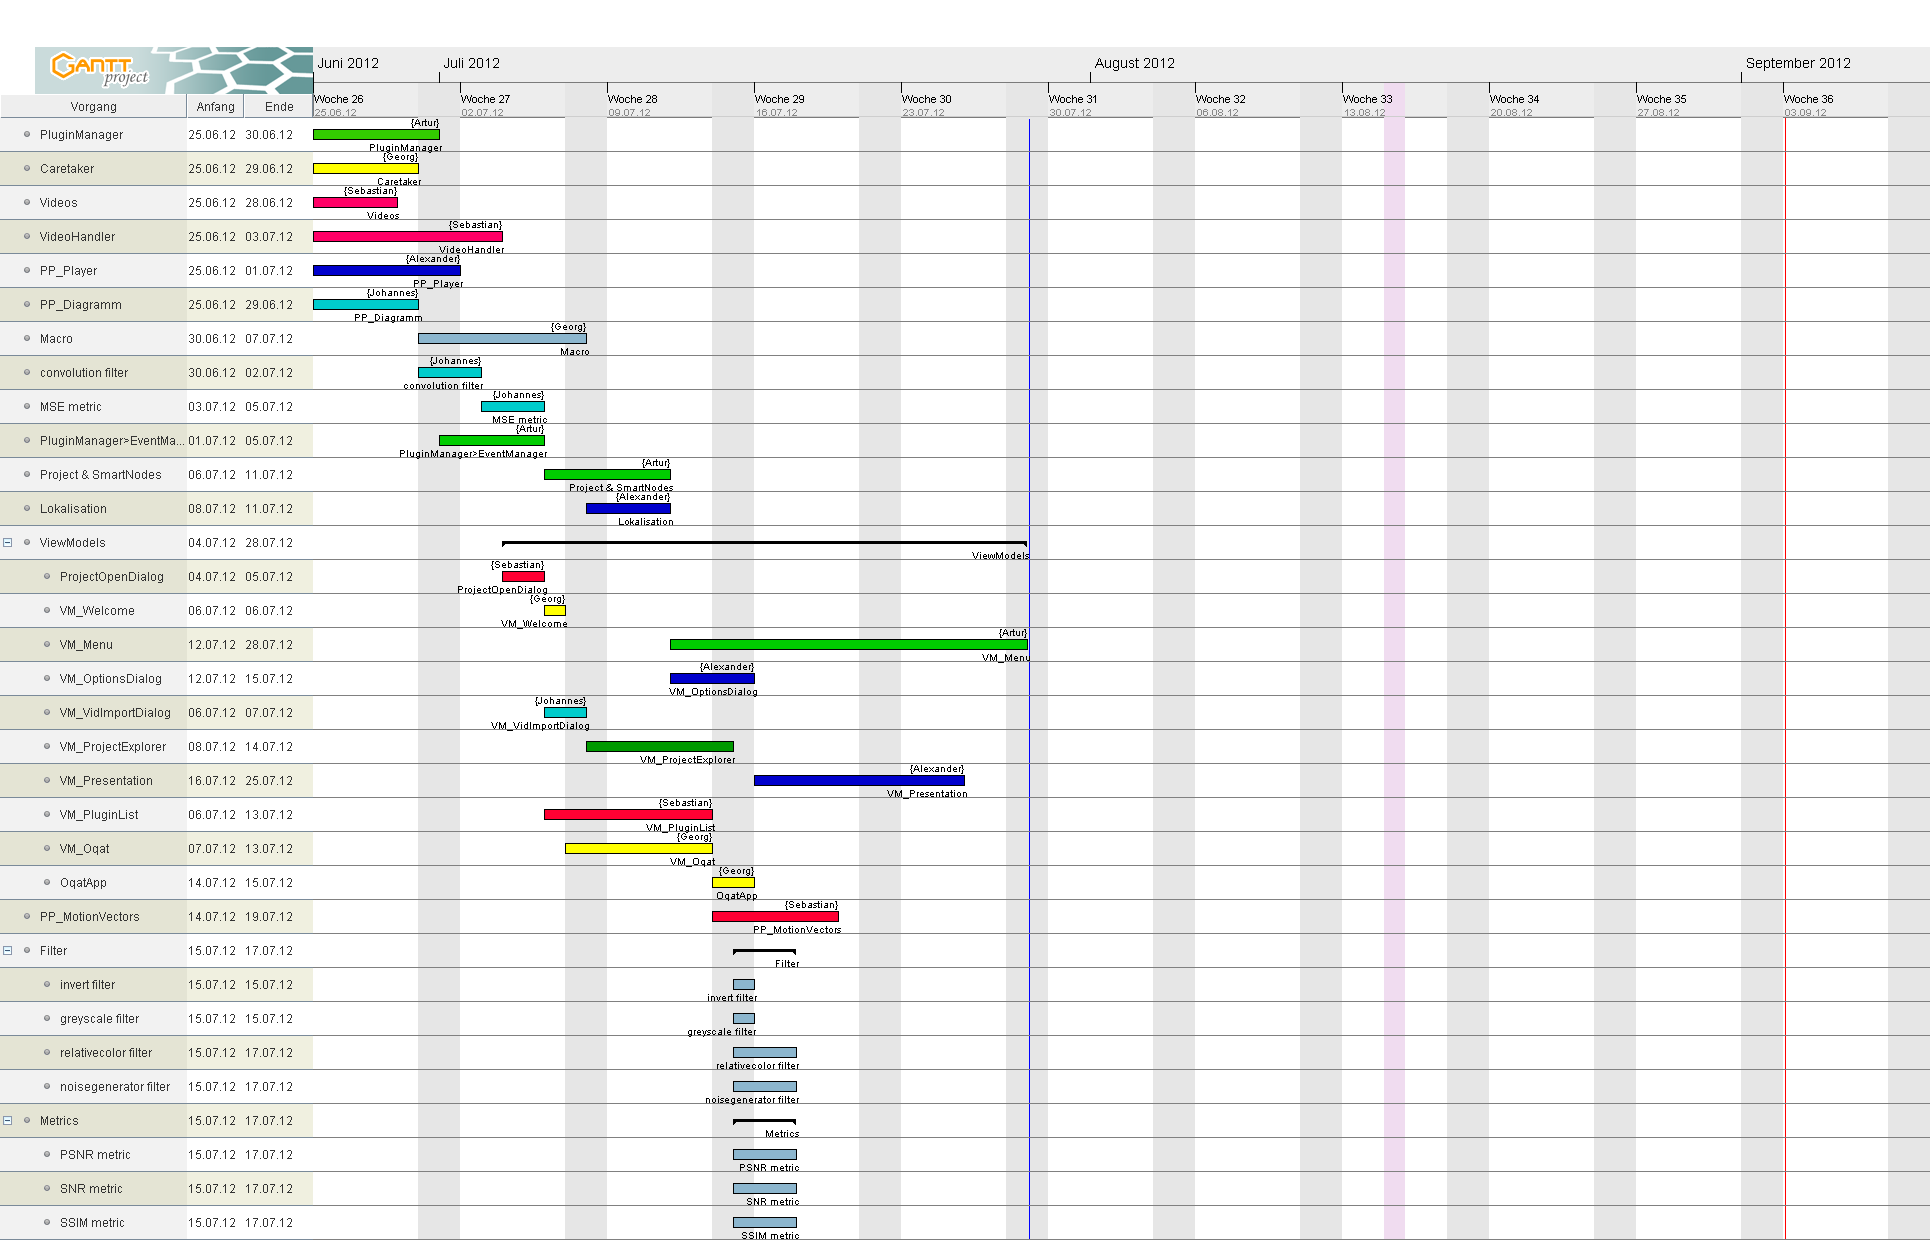
\includegraphics[scale=0.25]{bilder/gantt_planung.png}\\[5ex]
\caption{geplanter Implementierungsablauf}
\end{figure}

\begin{figure}
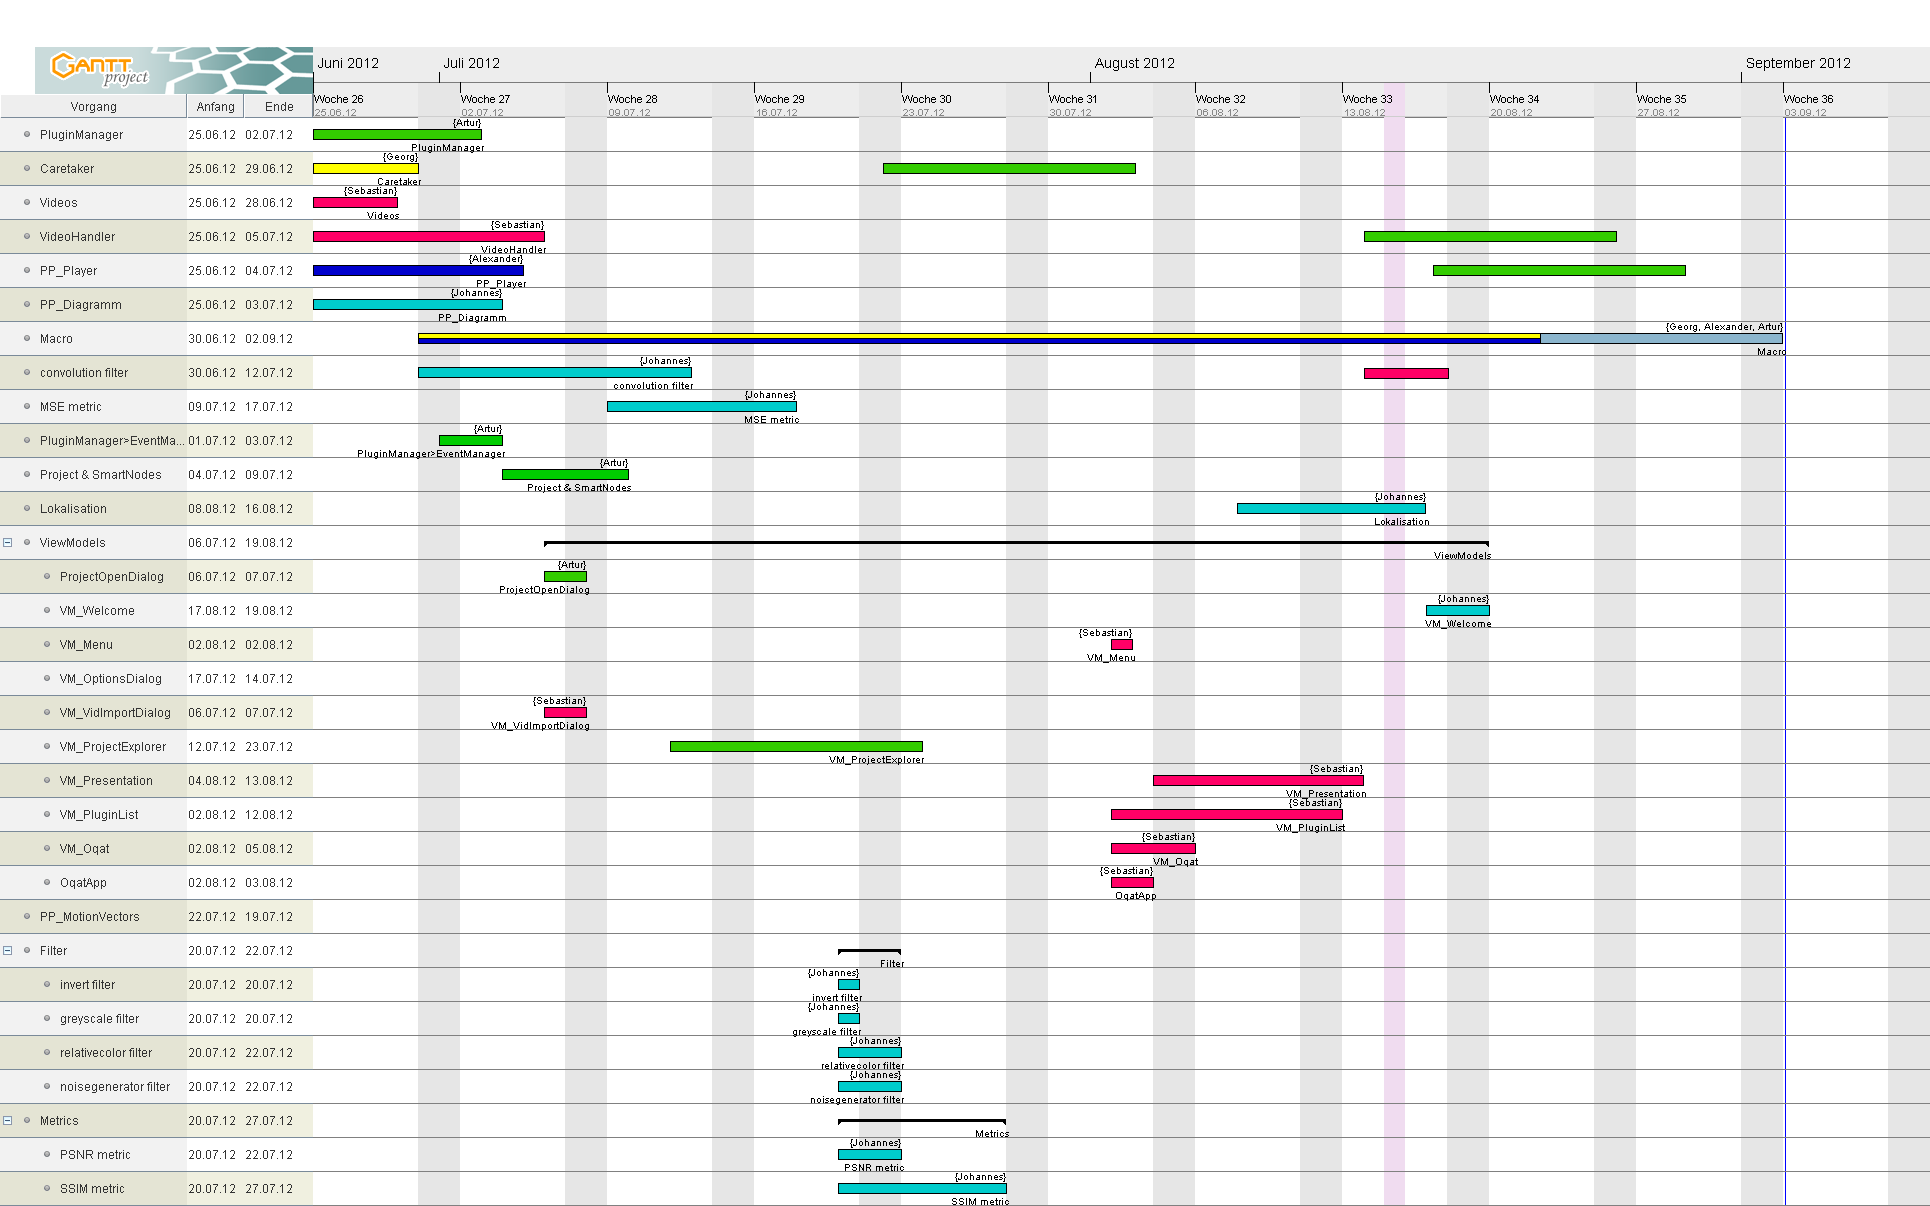
\includegraphics[scale=0.25]{bilder/gantt_tatsaechlich.png}\\[5ex]
\caption{ungefährer tatsächlicher Implementierungsablauf}
\end{figure}


\begin{figure}
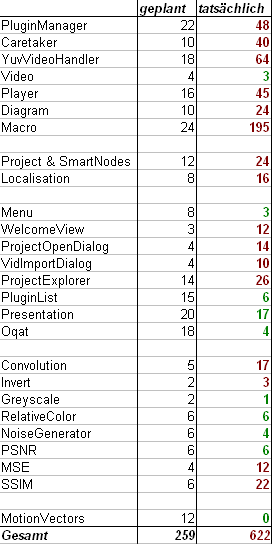
\includegraphics[scale=0.55]{bilder/planung_tabelle.png}\\[5ex]
\caption{Vergleich des erwarteten und tatsächlich Aufwands in Stunden}
\end{figure}